\section{Preconditioners}

Let $A$ be s.p.d.\ and suppose we are solving $A\vec{x}=\vec{b}$. Suppose we have some matrix $P$ with $P\approx A$. Then, the preconditioned linear system is

\begin{equation*}
    P^{-1}A\vec{x} = P^{-1}\vec{b},
\end{equation*}
where $P$ is called the preconditioner. There are two properties that are required of a good preconditioner

\begin{enumerate}[1)]
    \item $P^{-1}$ can be applied efficiently.
    \item $P\approx A$ or $P^{-1}A\approx I$
\end{enumerate}

%% Lecture 34

Our second requirement for the preconditioner $P$ is that $P \approx A$ or $P^{-1}A \approx I$. This condition can also be phrased as

\begin{enumerate}[a)]
    \item $\kappa(P^{-1}A) \ll \kappa(A)$ where $\kappa(A)$ is the condition number of $A$.
    \item The eigenvalues of $P^{-1}A$ are much more clustered than the eigenvalues of $A$.
    \item CG for $P^{-1}A$ requires much fewer iterations than CG applied to $A$.
\end{enumerate}

The two most extreme ``preconditioners" are $P=A$ and $P=I$. If $P=I$, then we satisfy condition 1 trivially, but not condition 2. If $P=A$, then we satisfy condition 2, but not condition 1. A good preconditioner is somewhere inbetween.

Because of the required spd property of CG, some careful algebra is required to apply CG to a preconditioned linear system. This is because, even if $P$ and $P^{-1}$ are symmetric, we have

\begin{equation*}
    (P^{-1}A)^T = A^T P^{-T} = AP^{-1}
\end{equation*}

$\Rightarrow P^{-1}A$ is symmetric iff $A$ and $P^{-1}$ commute.

There is a fix for this issue, and the result is the preconditioned CG (pCG) method:
%
\begin{algorithm}[H]
    \caption{Preconditioned Conjugate Gradient Method}
\begin{algorithmic}
    \STATE $\vec{r}^{\,(0)} =\vec{b}- A \vec{x}^{\,(0)}  $
    \STATE $\vec{d}^{\,(0)} = P^{-1}\vec{b}$
    \FOR{$i=0, 1, \ldots, n-1$}
        \STATE $\alpha^{(i)}=\frac{\vec{r}^{\,(i)T}P^{-1}\vec{r}^{\,(i)}}
        {\vec{d}^{\,(i)T}A\vec{d}^{\,(i)}}$
        \STATE $\vec{x}^{\,(i+1)} = \vec{x}^{\,(i)} + \alpha^{(i)}\vec{d}^{\,(i)}$
        \STATE $\vec{r}^{\,(i+1)} = \vec{r}^{\,(i)} - \alpha^{(i)}A\vec{d}^{\,(i)}$
        \STATE $\beta^{(i+1)} = \frac{\vec{r}^{\,(i+1)T}P^{-1}\vec{r}^{\,(i+1)}} {\vec{r}^{\,(i)T}P^{-1}\vec{r}^{\,(i)}}$
        \STATE $\vec{d}^{\,(i+1)} = P^{-1}\vec{r}^{\,(i+1)} + \beta^{(i+1)}\vec{d}^{\,(i)}$
    \ENDFOR
\end{algorithmic}
\end{algorithm}

If $P^{-1}$ can be applied (matvec) efficiently, the reduction of the number of iterations of CG may be large enough to offset the cost of applying $P^{-1}$.

Some of the most common preconditioners are:
\begin{enumerate}[1)]
    \item $P = \text{diag}(A)$
    \item A sparse approximate inverse (SPAI) matrix minimizes $||AT-I||_{\mathcal{F}}$, where $||\cdot||_{\mathcal{F}}$ is the Frobenius norm.
    \begin{equation*}
        ||A||_{\mathcal{F}} = \sum_{i=1}^{n}\sum_{j=1}^{m}a_{ij}^2
    \end{equation*}

This minimizer is a preconditioner $P^{-1}$, and the minimization is done over some sparsity pattern.

\begin{equation*}
    P^{-1} = \text{argmin}||AT-I||_{\mathcal{F}}
\end{equation*}

\item The Incomplete LU (ILU) factorization is an approximation LU decomposition of $A$. One version of the ILU drops all entries of the LU factorization of $A$ that are below some threshold. Therefore
\begin{equation*}
    A \approx LU
\end{equation*}
and we let $P=LU$. To apply $P^{-1}$, we need to Solvers
\begin{equation*}
    LU \vec{x} = \vec{b}.
\end{equation*}
This is done by solving
\begin{equation*}
    L\vec{y}=\vec{b} \quad \text{ and then } \quad U\vec{x} = \vec{y}
\end{equation*}
\item The multigrid algorithm we studied approximately solves $A\vec{x} = \vec{b}$ for certain matrices $A$.
We define the preconditioner as
\begin{equation*}
    P^{-1}\vec{b} := \text{GMG}(\vec{b})
\end{equation*}
where GMG($\vec{b}$) means applying some $\mu$-cycle with
some number of pre and post smoothing steps.

\item Domain Decomposition

\end{enumerate}

\section*{Domain Decomposition}

Here, we will focus on preconditioners for solving a standard second-order discritization of the elliptic PDE

\begin{align*}
    - \nabla \cdot (a(\vec{x})\nabla u) &= f(\vec{x})  & \vec{x} &\in \Omega\\
    u&=0 & \vec{x} &\in \partial \Omega
\end{align*}
we will write the linear system as $A\vec{x}=\vec{b}$

%% Lecture 35

This linear system $A\vec{x}=\vec{b}$ will be symmetic positive definite if $a(\vec{x})$ has some appropriate conditions. If we let $a(\vec{x})=1$, then

\begin{equation*}
    -\nabla \cdot ( a(\vec{x}) \nabla u )= \nabla \cdot (\nabla u) = -\Delta u = f
\end{equation*}

So, if you want, you can think of our PDE of interest to be the Poisson equation

\begin{align*}
    -\Delta u &=f &&\vec{x} \in \Omega \\
    u &= 0 &&\vec{x}\in \partial \Omega
\end{align*}

Domain Decomposition (DD) can be thought of as being a generalization of a block-Jacobi preconditioner. The block Jacobi precondition partitions the index set $I=\{1, \ldots, n\}$ as

\begin{equation*}
    I = I_1 \cup I_2 \cup \cdots \cup I_M
\end{equation*}
where each of the $I_i$'s are mutually disjoint. Then, the block Jacobi preconditioner is

\begin{equation*}
    P = (p_{ij})_{i, j=1, \ldots, n}
\end{equation*}
with
\begin{equation*}
    p_{ij} = \begin{cases}
    a_{ij} & \text{if $i$ and $j$ are in the same index set}\\
    0 & \text{Otherwise.}
\end{cases}
\end{equation*}

\begin{tikzpicture}
    \matrix[
    matrix of math nodes,
    nodes in empty cells,
    left delimiter={[},
    right delimiter={]},
    ](A){
    2&-1&&&&&\\
    -1&2&-1&&&&\\
    &-1&2&-1&&&\\
    &&-1&2&-1&&\\
    &&&-1&2&-1&\\
    &&&&-1&2&-1\\
    &&&&&-1&2\\
    };
    \node[left=.5em of A](){$A=$};
    \node[right=of A-1-7](){$I_1=\{1, 2\}$};
    \node[right=of A-4-7](){$I_2=\{3, 4\}$};
    \node[right=of A-7-7](){$I_3=\{5, 6, 7\}$};
    \node[font=\Huge]() at (A-2-6) {0};
    \node[font=\Huge]() at (A-6-2) {0};
\end{tikzpicture}

\begin{tikzpicture}
    \matrix[
    matrix of nodes,
    nodes in empty cells,
    left delimiter={[},
    right delimiter={]},
    every node/.style={minimum size=1.5em, anchor=center}
    ](P){
    2&-1&&&&&\\
    -1&2&&&&&\\
    &&2&-1&&&\\
    &&-1&2&&&\\
    &&&&2&-1&0\\
    &&&&-1&2&-1\\
    &&&&0&-1&2\\
    };
    \node[left=.5em of P](){$\Rightarrow P = $};
    \node[font=\Huge]() at (P-2-6) {0};
    \node[font=\Huge]() at (P-6-2) {0};
    \begin{scope}[red]

    \draw[decoration={brace, mirror}, decorate] (P-1-1.north west) -- (P-2-1.south west);
    \draw[decoration={brace}, decorate] (P-1-2.north east) -- (P-2-2.south east);

    \draw[decoration={brace, mirror}, decorate] (P-3-3.north west) -- (P-4-3.south west);
    \draw[decoration={brace}, decorate] (P-3-4.north east) -- (P-4-4.south east);

    \draw[decoration={brace, mirror}, decorate] (P-5-5.north west) -- (P-7-5.south west);
    \draw[decoration={brace}, decorate] (P-5-7.north east) -- (P-7-7.south east);
    \end{scope}
\end{tikzpicture}


A major benefit of this preconditioner is that its inverse can be trivially applied in parallel. Unfortunately it isn't very useful for large $n$ as it doesn't significantly reduce the number of CG iterations.

The problem is that elliptic PDEs, like the one we are solving, couple all points $\vec{x}\in\Omega$. That is if $f$ is changed in some small region of $\Omega$, the $u$ changes everywhere in $\Omega$. However, if $f(x_i)$ is changed, only part of $\left(P^{-1}\vec{f}\right)$ will change. For discretizations of elliptic PDEs, it is important that the preconditioner couples all of the discretization points. One way to do this coupling is with DD. Let's write our PDE as

\begin{align*}
    Lu &=f &&\vec{x} \in \Omega \\
    u &= 0 &&\vec{x}\in \partial \Omega
\end{align*}

If you want, think of $L=-\Delta$. We partition $\Omega$ as $\Omega=\Omega_1 \cup \Omega_2$ with overlap. That is, $\Omega_1 \cap \Omega_2 \neq \emptyset$. Upon discretization, the points in $\Omega_1$ are in some index set $I_1$, and the points in $\Omega_2$ are in some index set $I_2$. Letting $n_1$ and $n_2$ be the number of points in $\Omega_1$ and $\Omega_2$ respectively, we have
\begin{equation*}
    n_1 + n_2 > n
\end{equation*}
where $n$ is the total number of discretization points.

\begin{tikzpicture}
\matrix
[matrix of nodes,
every node/.style={
    fill,
    red,
    circle,
    inner sep=0,
    minimum size=5pt
},
row sep = 1em,
column sep = 1em,
]
(Omega)
{
&&&&\ &\ &\ &\ \\
&&&&\ &\ &\ &\ \\
&&&&\ &\ &\ &\ \\
&&&&\ &\ &\ &\ \\
\ &\ &\ &\ &\ &\ &\ &\ \\
\ &\ &\ &\ &\ &\ &\ &\ \\
\ &\ &\ &\ &\ &\ &\ &\ \\
\ &\ &\ &\ &\ &\ &\ &\ \\
};

\draw[line width=1.5mm, Green, opacity=.5]
    ([xshift=-0.5em, yshift=-0.5em] Omega-8-5.south west)
    rectangle
    ([xshift= 0.5em, yshift= 0.5em] Omega-1-8.north east);

\draw[line width=1.5mm, Magenta, opacity=.5]
    ([xshift=-0.5em, yshift=-0.5em] Omega-8-1.south west)
    rectangle
    ([xshift= 0.5em, yshift= 0.5em] Omega-5-8.north east);

\node[above=of Omega-5-2](){$\Omega$};
\node[left=1em of Omega-7-1, fill=Magenta, opacity=0.5, text opacity=1, circle](){$\Omega_1$};
\node[above=1em of Omega-1-7, fill=Green, opacity=0.5, text opacity=1, circle](){$\Omega_2$};

\draw [thick]
    ([xshift=-0.5em, yshift=-0.5em] Omega-8-1.south west)
  --([xshift=-0.5em, yshift= 0.5em] Omega-5-1.north west)
  --([xshift=-0.5em, yshift= 0.5em] Omega-5-5.north west)
  --([xshift=-0.5em, yshift= 0.5em] Omega-1-5.north west)
  --([xshift= 0.5em, yshift= 0.5em] Omega-1-8.north east)
  --([xshift= 0.5em, yshift=-0.5em] Omega-8-8.south east)
  --cycle;

\draw[<-] (Omega-1-8) to[bend left=10] (3,2) node[right]{This point's index is in $I_2$};
\draw[<-] (Omega-8-3) to[out=-90, in=200] (3,-2) node[right]{This point's index is in $I_1$};
\draw[<-] (Omega-5-7) to[out=45, in=180] (3,0) node[right]{This point's index is in $I_1$ and $I_2$};


\end{tikzpicture}

%% Lecture 36
We can describe DD at the continuous level, or at the discretize level. To be applied at the discrete level, we require a restriction and prolongation operators. For each $I_i$, we define a $n \times n_i$ rectangular matrix $R_i^T$ such that

\begin{equation*}
    (R_i^T \vec{x})_k = \begin{cases}
        x_k & \text{ if } k\in I_i\\
        0 & \text{ if } k \notin I_i \qquad k=1, \ldots, n
\end{cases}
\end{equation*}

\underline{Ex}

If $I_1=\{ 1, 2, 3, 4 \}$ and  $I_2 = \{ 4, 5, 6 \}$, then

\begin{equation*}
    R_1^T =
    \begin{bmatrix}
            1 & 0 & 0 & 0 \\
            0 & 1 & 0 & 0 \\
            0 & 0 & 1 & 0 \\
            0 & 0 & 0 & 1 \\
            0 & 0 & 0 & 0 \\
            0 & 0 & 0 & 0 \\
    \end{bmatrix},
    \qquad
    R_2^T =
    \begin{bmatrix}
            0 & 0 & 0 \\
            0 & 0 & 0 \\
            0 & 0 & 0 \\
            1 & 0 & 0 \\
            0 & 1 & 0 \\
            0 & 0 & 1 \\
    \end{bmatrix}
\end{equation*}

Then, the matrices $R_1$ and $R_2$ are restriction operations that remove all entries from $\vec{x}$ except those indexed in $I_i$. For example

\begin{equation*}
    R_1
    \begin{bmatrix}
        x_1\\x_2\\\vdots\\x_6
    \end{bmatrix}
=
\begin{bmatrix}
        1 & 0 & 0 & 0 & 0 & 0\\
        0 & 1 & 0 & 0 & 0 & 0\\
        0 & 0 & 1 & 0 & 0 & 0\\
        0 & 0 & 0 & 1 & 0 & 0\\
\end{bmatrix}
    \begin{bmatrix}
        x_1\\x_2\\x_3\\ x_4\\ x_5 \\x_6
    \end{bmatrix}
    =
    \begin{bmatrix}
        x_1\\x_2\\x_3\\ x_4
    \end{bmatrix}
    \qquad
    R_2
    \begin{bmatrix}
        x_1\\x_2\\\vdots\\x_6
    \end{bmatrix}
    =
    \begin{bmatrix}
        x_4\\x_5\\x_6
    \end{bmatrix}
\end{equation*}

Then, the local subdomain matrices

\begin{equation*}
    A_1 = R_1 A R_1^T, \qquad A_2 = R_2AR_2^T
\end{equation*}

\begin{tikzpicture}
    \matrix[
    matrix of math nodes,
    nodes in empty cells,
    left delimiter={[},
    right delimiter={]},
    ](A){
    2&-1&&&&&\\
    -1&2&-1&&&&\\
    &-1&2&-1&&&\\
    &&-1&2&-1&&\\
    &&&-1&2&-1&\\
    &&&&-1&2&-1\\
    &&&&&-1&2\\
    };
    \node[left=.5em of A](){$A=$};
    \node[font=\Huge]() at (A-2-6) {0};
    \node[font=\Huge]() at (A-6-2) {0};
\end{tikzpicture}

\begin{equation*}
    R_1AR_1^T =
\begin{bmatrix}
        1 & 0 & 0 & 0 & 0 & 0\\
        0 & 1 & 0 & 0 & 0 & 0\\
        0 & 0 & 1 & 0 & 0 & 0\\
        0 & 0 & 0 & 1 & 0 & 0\\
\end{bmatrix}
\begin{tikzpicture}[baseline=(current bounding box.center)]
    \matrix[
    matrix of math nodes,
    nodes in empty cells,
    left delimiter={[},
    right delimiter={]},
    ](A){
    2&-1&&&&&\\
    -1&2&-1&&&&\\
    &-1&2&-1&&&\\
    &&-1&2&-1&&\\
    &&&-1&2&-1&\\
    &&&&-1&2&-1\\
    &&&&&-1&2\\
    };
    \node[font=\Huge]() at (A-2-6) {0};
    \node[font=\Huge]() at (A-6-2) {0};
\end{tikzpicture}
    \begin{bmatrix}
            1 & 0 & 0 & 0 \\
            0 & 1 & 0 & 0 \\
            0 & 0 & 1 & 0 \\
            0 & 0 & 0 & 1 \\
            0 & 0 & 0 & 0 \\
            0 & 0 & 0 & 0 \\
    \end{bmatrix}
\end{equation*}

\begin{equation*}
    =
\begin{bmatrix}
        1 & 0 & 0 & 0 & 0 & 0\\
        0 & 1 & 0 & 0 & 0 & 0\\
        0 & 0 & 1 & 0 & 0 & 0\\
        0 & 0 & 0 & 1 & 0 & 0\\
\end{bmatrix}
\begin{bmatrix}
    2&-1&0&0\\
    -1&2&-1&0\\
    0&-1&2&-1\\
    0&0&-1&2\\
    0&0&0&-1&\\
    0&0&0&0\\
\end{bmatrix}
=
\begin{bmatrix}
    2&-1&0&0\\
    -1&2&-1&0\\
    0&-1&2&-1\\
    0&0&-1&2\\
\end{bmatrix}
\end{equation*}

The idea of DD is to solve discretizations of the PDE in each subdomain $\Omega_1$ and $\Omega_2$. However, since boundary conditions are required on the boundaries of $\Omega_1$ and $\Omega_2$, and part of these boundaries are in the interior of $\Omega$.

\begin{center}
\begin{tikzpicture}
\draw[pattern=north west lines, pattern color=Green, dashed, draw=Green, ultra thick] (2,0) rectangle (4,4);
\draw[pattern=north east lines, pattern color=Red, dashed, draw=Red, ultra thick] (0,0) rectangle (4,2);
\draw[thick](0, 0) -- (0, 2) -- (2, 2) -- (2, 4) -- (4, 4) -- (4, 0) -- cycle;

\node()at(1, 3){$\Omega$};
\node[Green, fill=white, circle]()at(3, 3){$\Omega_2$};
\node[Red, fill=white, circle]()at(1, 1){$\Omega_1$};
\draw[->, thick] (1.5, -.5) node[anchor=north, Green]{$\Gamma_2$} to[bend left=30] (2, 0.5);
\draw[->, thick] (4.5, 1.5) node[anchor=west, Red]{$\Gamma_1$} to[bend left=30] (3.5, 2);
\end{tikzpicture}
\end{center}

Letting $\Gamma_1$ and $\Gamma_2$ be the boundaries of $\Omega_1$ and $\Omega_2$ that are in the interior of $\Omega$, the DD method starts with some $u^0$ and iterates by solving

\begin{equation*}
    \begin{cases}
    Lu_1^{k+1} = f & \vec{x}\in \Omega_1\\
    u_1^{k+1} = u_2^k \bigg\rvert_{\Gamma_1} & \vec{x}\in \Gamma_1 \\
    u_1^{k+1} = 0 & \vec{x} \in \partial \Omega_1 \setminus \Gamma_1
    \end{cases}
\end{equation*}

\begin{equation*}
    \begin{cases}
    Lu_2^{k+1} = f & \vec{x}\in \Omega_2\\
    u_2^{k+1} = u_1^{k+1} \bigg\rvert_{\Gamma_2} & \vec{x}\in \Gamma_2 \\
    u_2^{k+1} = 0 & \vec{x} \in \partial \Omega_2 \setminus \Gamma_2
    \end{cases}
\end{equation*}

Note the notation

\begin{center}

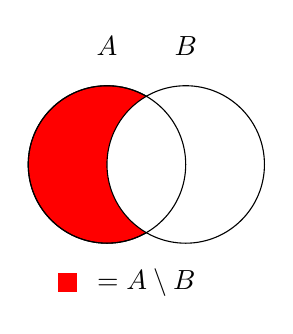
\begin{tikzpicture}
\draw[fill=Red] (0, 0) circle (1);
\draw[fill=White] (1, 0) circle (1);
\draw  (0, 0) circle (1);
\node()at(0, 1.5){$A$};
\node()at(1, 1.5){$B$};
\node()at(.5, -1.5){$=A\setminus B$};
\node[minimum size=5pt, fill=Red]()at(-0.5, -1.5){};
\end{tikzpicture}
\end{center}

With some conditions on $L$ (coercivity), this iterative method converges in some norm to the exact solution. The convergence is geometric, meaning that

\begin{equation*}
    || u-u^k|| \leq \rho^k || u-u_0||
\end{equation*}
where $\rho<1$ depends on the choice of $\Omega_1$ and $\Omega_2$

%% Lecture 37

This DD method cna be written in another form by using the residual. We will do this for 2 index sets partitioning $\{ 1, \ldots, n \}$ with overlap. At iteration $k$, the residual is

\begin{equation*}
    \vec{r}^{\, k} = \vec{f} - A\vec{x}^{\, k}
\end{equation*}
and the error satisfies

\begin{equation*}
    \vec{x} = \vec{x}^{\, k} + \vec{e}^{\, k}
\end{equation*}

Multiply both sides by $A$,

\begin{align*}
    A\vec{x} &= A\vec{x}^{\, k} + A\vec{e}^{\, k}\\
    \Rightarrow \vec{f} &= A\vec{x}^{\, k} + A\vec{e}^{\, k}\\
    \Rightarrow A\vec{e}^{\, k} &=\vec{f} - A\vec{x}^{\, k} \\
    \Rightarrow A\vec{e}^{\, k} &=\vec{r}^{\, k}
    \Rightarrow \vec{e}^{\, k} =A^{-1}\vec{r}^{\, k}
\end{align*}
To update the solution at indicies in $I_1$, we need to restrict the residual to $I_1$. Once we've solved for the error on $I_1$, we prolong the error back to all the indices. We then repeat for $I_2$.

\begin{align*}
    \vec{x}^{\, k + 1/2} &= \vec{x}^{\, k} +
    R_1^T A_1^{-1} R_1
    \left(\vec{f} - A\vec{x}^{\, k}\right)\\
    \vec{x}^{\, k + 1} &= \vec{x}^{\, k + 1/2} +
    R_2^T A_2^{-1} R_2
    \left(\vec{f} - A\vec{x}^{\, k + 1/2}\right)\\
\end{align*}

Letting

\begin{equation*}
    P_i := R_i^T A_i^{-1} R_i A, \qquad i=1,2
\end{equation*}

we have

\begin{align*}
    \vec{x}^{\, k + 1/2} &= (I - P_1)\vec{x}^{\, k} +
    R_1^T A_1^{-1} R_1\vec{f},\\
    \vec{x}^{\, k + 1} &=(I - P_2) \vec{x}^{\, k + 1/2} +
    R_2^T A_2^{-1} R_2 \vec{f}
\end{align*}

Therefore, the convergence of this method depends on the eigenvalues of the iteration matrix. For this algorithm, it can be found as follows.

\begin{align*}
    \vec{x}^{\, k + 1} &= (I - P_2) \left((I - P_1)\vec{x}^{\, k} +
    R_1^T A_1^{-1} R_1\vec{f}\right) +
    R_2^T A_2^{-1} R_2 \vec{f}\\
    &= (I - P_2)(I - P_1) \vec{x}^{\, k}+ \vec{g}
\end{align*}
where
\begin{align*}
    \vec{g}&=(I - P_2)R_1^T A_1^{-1} R_1\vec{f} + R_2^T A_2^{-1} R_2 \vec{f}\\
    \Rightarrow \vec{x}^{\, k + 1} &= M\vec{x}^{\, k} + \vec{g}
\end{align*}
which is the iteration matrix.

Since the iteration matrix depends on a product, this method is called a \emph{Multplicative Schwarz iteration}.

Instead, we can use the last iterate $\vec{x}^{\, k}$ in both subdomains. That is,


\begin{align*}
    \vec{x}^{\, k + 1/2} &= \vec{x}^{\, k} +
    R_1^T A_1^{-1} R_1
    \left(\vec{f} - A\vec{x}^{\, k}\right)\\
    \vec{x}^{\, k + 1} &= \vec{x}^{\, k + 1/2} +
    R_2^T A_2^{-1} R_2
    \left(\vec{f} - A\vec{x}^{\, k}\right)\\
\end{align*}

Then, applying $A_1^{-1}$ and $A_2^{-1}$ can be done in parallel rather than sequenctially. Putting the iterates together

\begin{align*}
    \vec{x}^{\, k + 1} = \vec{x}^{\, k} +
    \left(R_1^T A_1^{-1} R_1 + R_2^T A_2^{-1} R_2\right)
    \left(\vec{f} - A\vec{x}^{\, k}\right)\\
\end{align*}

Therefore, the iteration matrix is
\begin{align*}
    &I - \left(R_1^T A_1^{-1} R_1 + R_2^T A_2^{-1} R_2\right)A\\
    = &I -P_1-P_2
\end{align*}
and we call this method an \emph{Additive Schwarz method}.

There is an alternative way to think of additive Schwarz. Assuming we are at a fixed point $\vec{x}$, we have 


\begin{align*}
    \vec{x} &= \vec{x}+
    \left(R_1^T A_1^{-1} R_1 + R_2^T A_2^{-1} R_2\right)
    \left(\vec{f} - A\vec{x}\right)\\
    &\Rightarrow\left(R_1^T A_1^{-1} R_1 + R_2^T A_2^{-1} R_2\right)
    A\vec{x} = \left(R_1^T A_1^{-1} R_1 + R_2^T A_2^{-1} R_2\right)\vec{f}.\\
\end{align*}
Which is simply a preconditioned version of $A\vec{x} = \vec{f}$ with the preconditioner

\begin{equation*}
    P^{-1} = R_1^T A_1^{-1} R_1 + R_2^T A_2^{-1} R_2
\end{equation*}

%% Lecture 38

A problem with DD as presented is that it's convergence slows down when we have more than 2 processors (i.e.\ 2 subdomains). The reason is that not all the domains are talking to one another. As is, only neighboring domains communicate.

One solution is to use a two-scale DD method. That is, one grid size $h$ is used to solve problems on subdomains, and another grid with grid size $H$ couples the subdomains. This gives us 2 more parameters, the grid sizes, that play a role in the multi-level DD method.

Given an elliptic PDE in $\mathbb{R}^2$, we construct subdomains as follows:

\begin{center}
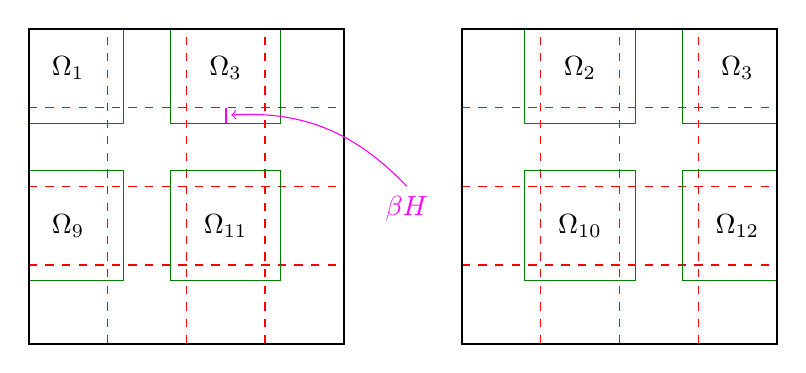
\begin{tikzpicture}
    \draw[dashed, red] (0, 0) grid (4,4);
    \draw[Green] (0, 4) rectangle (1.2, 2.8);
    \draw[Green] (1.8, 2.8) rectangle (3.2, 4);
    \draw[Green] (0, 2.2) rectangle (1.2, 0.8);
    \draw[Green] (1.8, 2.2) rectangle (3.2, 0.8);
    \draw[thick] (0, 0) rectangle (4, 4);
    \node[]() at (0.5, 3.5) {$\Omega_1$};
    \node[]() at (2.5, 3.5) {$\Omega_3$};
    \node[]() at (0.5, 1.5) {$\Omega_9$};
    \node[]() at (2.5, 1.5) {$\Omega_{11}$};

    \draw[thick, Magenta] (2.5, 2.8) -- (2.5, 3);

    \draw[<-, shorten <=2pt, Magenta] (2.5, 2.9) to[bend left=25](4.8, 2)
    node[below]{$\beta H$}
    ;
    \begin{scope}[xshift=5.5cm]
    \draw[dashed, red] (0, 0) grid (4,4);
    \draw[Green] (0.8, 4) rectangle (2.2, 2.8);
    \draw[Green] (2.8, 4) rectangle (4, 2.8);
    \draw[Green] (0.8, 2.2) rectangle (2.2, 0.8);
    \draw[Green] (2.8, 2.2) rectangle (4, 0.8);
    \draw[thick] (0, 0) rectangle (4, 4);
    \node[]() at (1.5, 3.5) {$\Omega_2$};
    \node[]() at (3.5, 3.5) {$\Omega_3$};
    \node[]() at (1.5, 1.5) {$\Omega_{10}$};
    \node[]() at (3.5, 1.5) {$\Omega_{12}$};
    \end{scope}
\end{tikzpicture}
\end{center}

An additive Schwarz preconditioner is

\begin{equation*}
    P^{-1} = M_{AS, 1} = \sum_{i=1}^{16} R_i^TA_i^{-1}R_i
\end{equation*}
However, not all subdomains are coupled. If we define $R_H^T$ to be an interpolation map as in GMG from the coarse grid to the fine grid. Then $R_H$ is a restriction map. Then, a two-grid additive Schwarz preconditioner is

\begin{equation*}
    P^{-1} = M_{AS, 2} = R_H^TA_H^{-1}R_H+\sum_{i=1}^{16} R_i^TA_i^{-1}R_i
\end{equation*}

and

\begin{equation*}
    \text{cond}(M_{AS, 2}A) \leq C (1+\beta^{-1})
\end{equation*}
Where $C$ is independent of $h$ and $H$.
